\onecolumn
\section{Appendix}
Figure \ref{Fig:SimulinkModel} shows the Simulink model used to control the QArm Robot. The following sections are the Matlab Scrips used by the Simulink Model: 

\begin{figure}[htb]
\centering
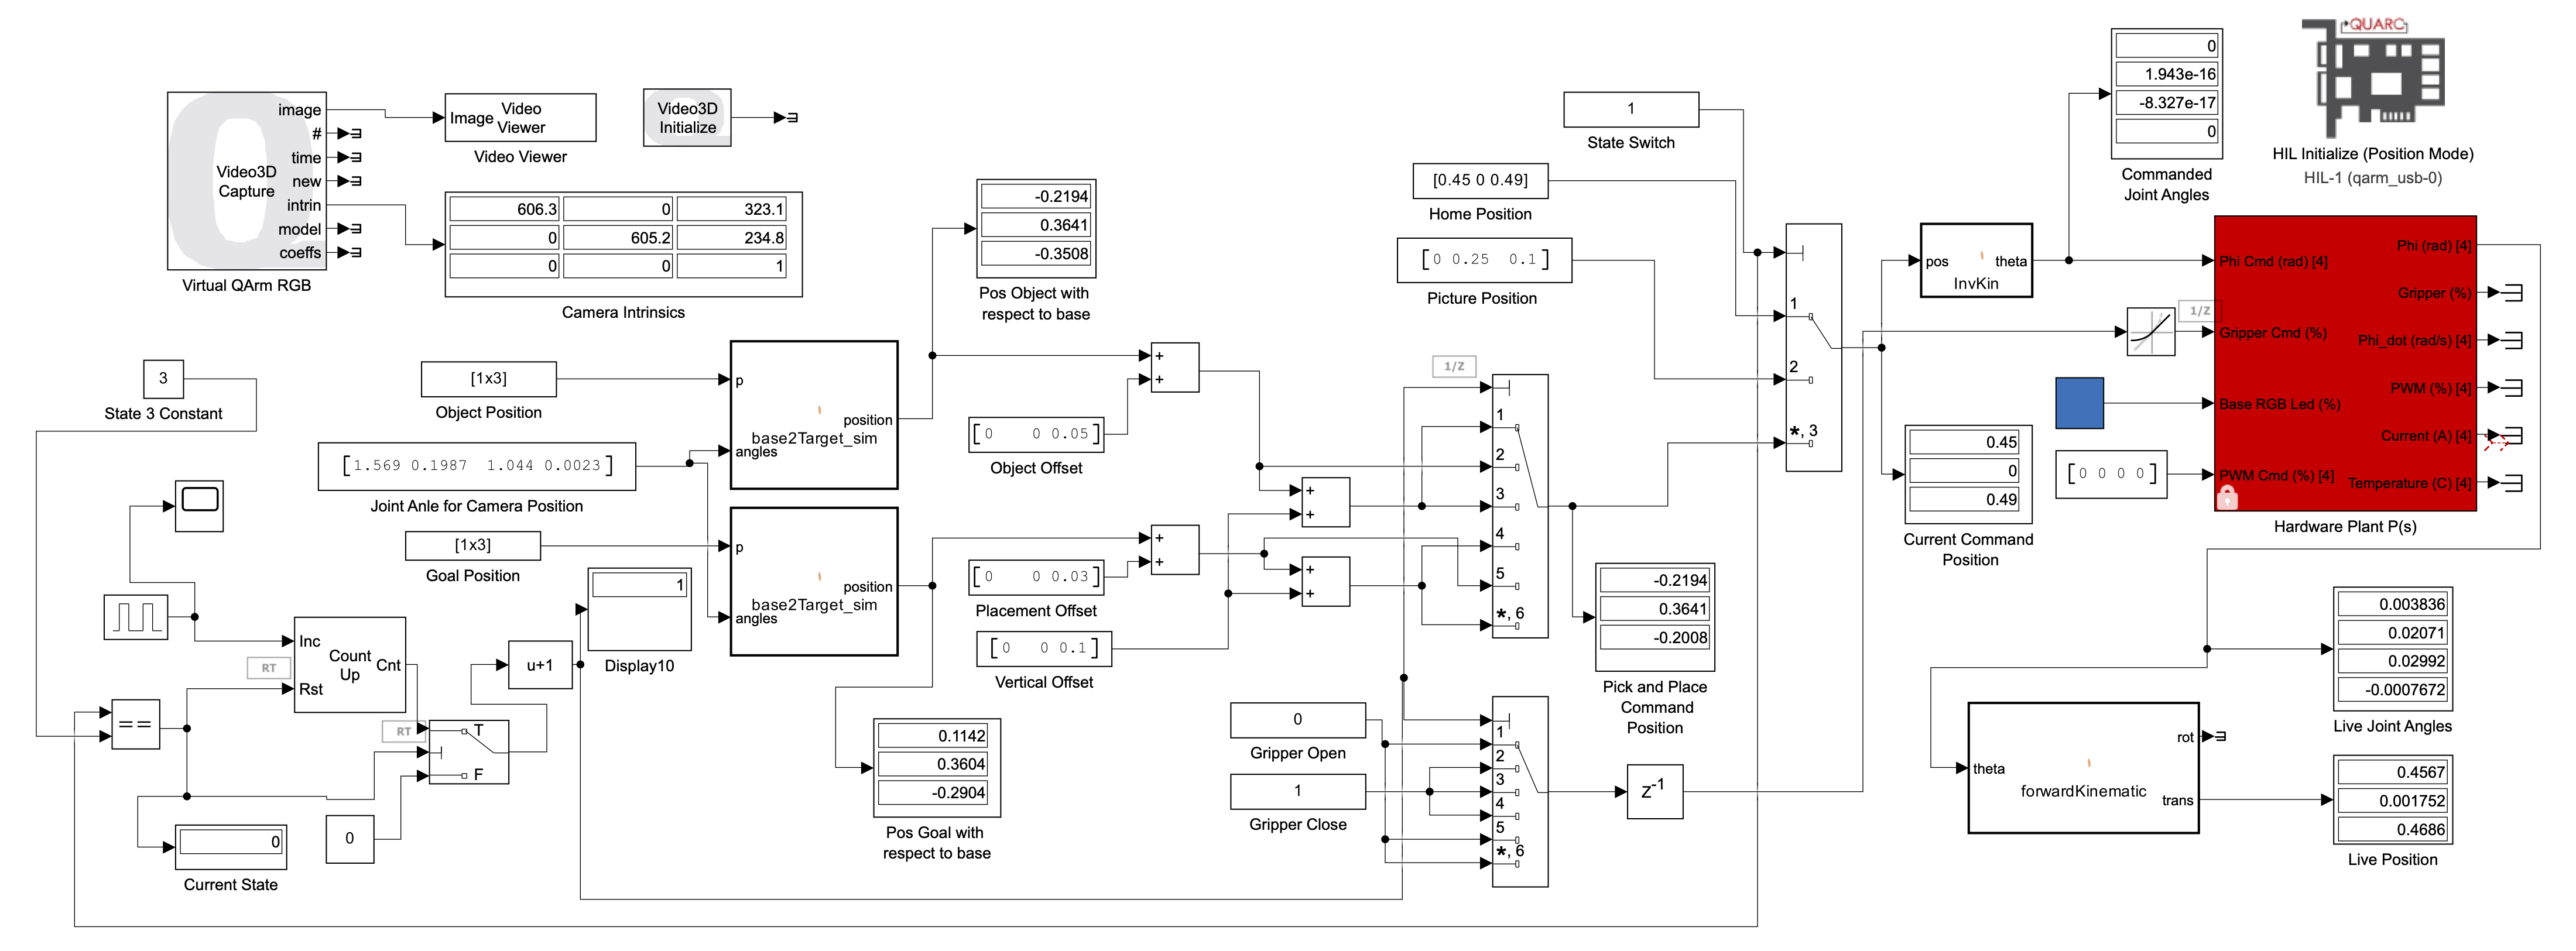
\includegraphics[width=\textwidth]{Figures/SimulinkModel.png}
\caption{Simulink Model}
\label{Fig:SimulinkModel}
\centering
\end{figure}

\subsection{base2Target.m}

\lstinputlisting[language=Matlab]{Code/base2Target.m}

\subsection{forwardKinematics.m}

\lstinputlisting[language=Matlab]{Code/forwardKinematics.m}

\subsection{homoTransform.m}

\lstinputlisting[language=Matlab]{Code/homoTransform.m}

\subsection{InverseHomogeneousMatrix.m}

\lstinputlisting[language=Matlab]{Code/InverseHomogeneousMatrix.m}

\subsection{InverseKinematic.m}

\lstinputlisting[language=Matlab]{Code/InverseKinematic.m}
